\documentclass[12pt, a4paper]{article}
\usepackage{graphicx}
%\usepackage[square,numbers]{natbib}
\usepackage{url}
\usepackage{amsmath}

\renewcommand{\refname}{Kaynakça}
\title{\textbf{GAN Metodu ile Yüz Oluşturma}}
\author{Elif Filiz}
\date{07.03.2024}
\begin{document}
	
	\thispagestyle{empty}
	\maketitle 
	
	\textbf{KÜTAHYA SAĞLIK BİLİMLERİ ÜNİVERSİTESİ}\centering
	\begin{figure}[!h]
		\centering
		
\includegraphics{ksbu}
	\end{figure}
	\newpage
	\tableofcontents
	\newpage
	\section{Giriş} 
		\raggedright
			\subsection{Yapay Zeka}
		Günümüzde, gerçekçi ve inandırıcı yüz sentezi, sanat, güvenlik, eğlence ve daha birçok alanda önemli uygulamalara sahiptir. Yapay zeka uygulamaları özellikle eğlence sektöründe sık sık kullanılmaktadır\cite{9628901}. Film endüstrisi veya diğer medya sektörlerinde, çözünürlüğü artırma gibi zorluklarla karşılaşıldığında, eski görüntülerin yeniden işlenerek daha yüksek çözünürlükte sunulması için Çekişmeli Üretici Ağlar (Generative Adversarial Networks - GAN) modeli olarak bilinen GAN kullanılabilmektedir\cite{8099502}. 
		
		\subsection{Gan Nedir?}
		GAN'lar, veri üretimi için rekabetçi bir yaklaşım sunar, birbirleriyle yarışan iki sinir ağı olan generative ve discriminative ağları içerir\cite{goodfellow2014generative}. Üretici (generative), rastgele gürültüden gerçekçi veriler üretmeye çalışır. Ayırt edici (discriminator) ise, gerçek verileri ve Üretici tarafından üretilen sahte verileri birbirinden ayırt etmeye çalışır. Discriminator, bu iki tür veriyi ayırt edebilmek için eğitilir. GAN’ın temel fikri, bu iki ağın karşıt görevlerde birbirlerini eğitmeleridir. Üretici, daha gerçekçi veriler üretebilmek için discriminator’un yanıltıcı verileri daha iyi ayırt etme yeteneğini geliştirmeye çalışırken, discriminator da gerçek ve sahte verileri daha iyi ayırt edebilmek için çalışır. Bu sürekli rekabet, her iki ağın performansını artırmalarına ve sonuç olarak Üretici, giderek daha gerçekçi veriler üretebilir hale gelir.

		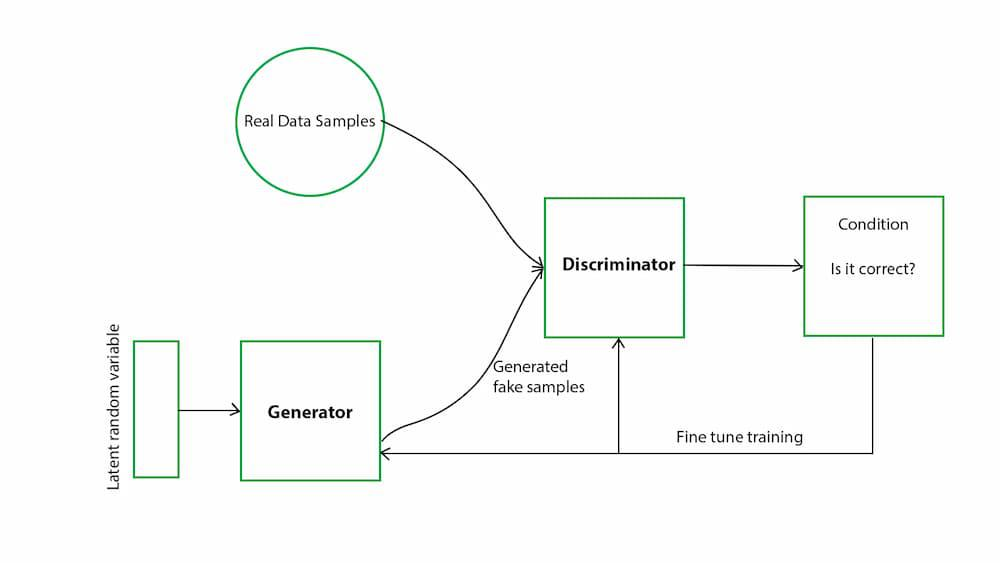
\includegraphics[width=1\textwidth]{gan}

		Generative'in görevi, görüntüler veya metinler gibi gerçek verilere çok benzeyen yeni veriler oluşturmaktır. Discriminative, gerçek veriler (bir eğitim veri kümesinden) ile Generative tarafından oluşturulan veriler arasında ayrım yapmaya çalışan bir eleştirmen gibi davranır.
		
		Generative girdi olarak rastgele bir gürültü vektörünü alır. Bu gürültü vektörü rastgele değerler içerir ve Generative'in yaratım sürecinin başlangıç noktası görevi görür. Generative, dahili katmanlarını ve öğrenilen kalıplarını kullanarak, gürültü vektörünü, oluşturulmuş bir görüntü gibi yeni bir veri örneğine dönüştürür.

		Discriminator iki tür girdi alır:
		Eğitim veri kümesinden gerçek veri örnekleri.
		Önceki adımda Generative tarafından oluşturulan veri örnekleri. Discriminator'ün görevi her girdiyi analiz etmek ve bunların gerçek veri mi yoksa Generative'in uydurduğu bir şey mi olduğunu belirlemektir. 0 ile 1 arasında bir olasılık puanı verir. 1 puanı, verinin muhtemelen gerçek olduğunu, 0 ise sahte olduğunu gösterir.
		Önemli olan sürekli gelişmektir. Eğer Discriminator sürekli olarak her şeyi doğru bir şekilde tanımlarsa, fazla bir şey öğrenmeyecektir. Yani amaç Generator'ün sonunda Discriminator'ü kandırmasıdır.
		
		\subsection{Proje}
		Yapay zeka diğer yandan, gerçekçi insan yüzlerini sentezlemek için geliştirilen yöntemler üzerinde odaklanmaktadır. Yüz oluşturma projeleri, yapay zeka teknolojilerinin derin öğrenme alanındaki önemli bir uygulama alanını temsil etmektedir. Ancak, bu alanda karşılaşılan temel bir zorluk, gerçekçi yüzlerin oluşturulması için de gereken yüksek çözünürlük ve detay düzeylerini elde etmek ve aynı zamanda bu yüzlerin inandırıcılığını korumaktır. Bu zorlukların üstesinden gelmek için, araştırmacılar ve mühendisler Generative Adversarial Networks (GAN) gibi derin öğrenme tekniklerini kullanmaktadır. Gan'ların kullandığı rekabetçi yaklaşım sayesinde, gerçeğe oldukça yakın görüntüler üretmek mümkün hale gelir. Diğer yandan güvenlik açısından bir tehdit olarak görülen sahte videoların oluşturulmasında da benzeri uygulamaların kullanıldığı görülmektedir\cite{masood2023deepfakes}. Yüz oluşturma projelerinde etik ve mahremiyet sorunları da önemli bir yer tutmaktadır. Zaman zaman, GAN'lar tarafından üretilen gerçekçi görüntülerin kötü niyetli amaçlarla kullanılması endişeleri gündeme gelmektedir. Bu nedenle, yüz oluşturma projelerinde güvenlik ve etik standartların dikkate alınması büyük önem taşımaktadır. Bunların yanı sıra var olmayan bir kişinin fotoğrafının oluşturulması, görüntüde belli	özelliklerin değiştirilerek farklı görüntülerin	üretilmesi gibi durumlarda GAN modelleri devreye girmektedir. 
		
		Bu rapor, yapay zeka destekli GAN yöntemlerinin kullanıldığı yüz oluşturma projelerinin detaylı bir incelemesini sunacak ve mevcut tekniklerin avantajlarını, karşılaşılan zorlukları ve bu alandaki gelecekteki potansiyeli ele alacaktır.
	
		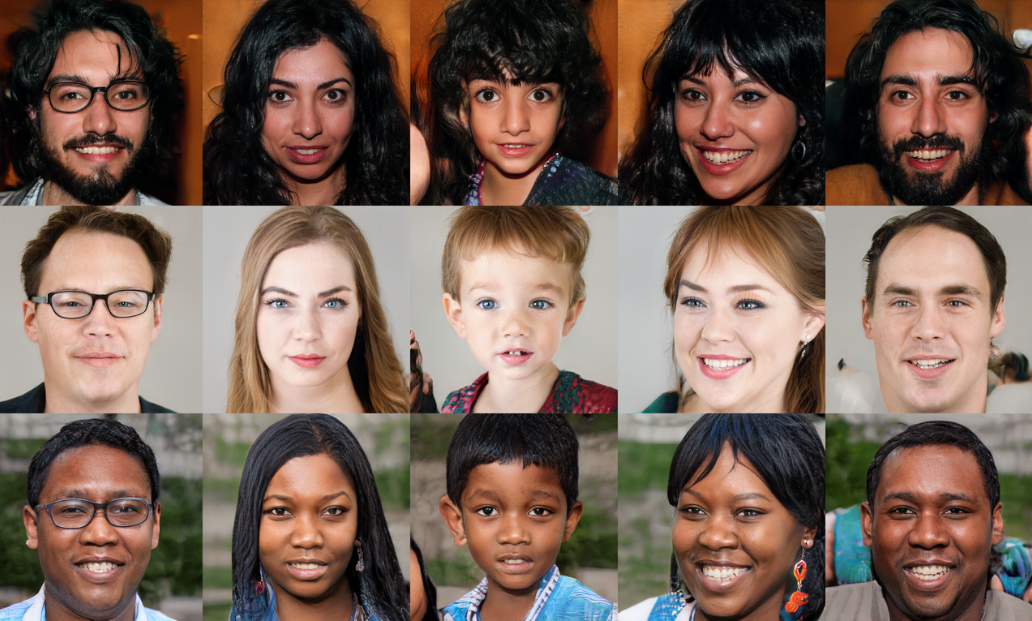
\includegraphics[width=1\textwidth]{abcd}

\begin{center}
		\section{Literatür Araştırması}
\end{center}
	\begin{flushleft}
	Yapılmış AI tabanlı yüz oluşturma uygulamalarında lider görülen "Generated Photos\cite{Generated-2024-03-08}" uygulamasıdır. Uygulama öncesinde oluşturulmuş seçenekler sunmakla birlikte yeni bir yüz oluşturma imkanı ve rastgele bir yüz üreteci imkanı da sunuyor. Öncelikle cinsiyet seçimi sonrası pozisyon belirleniyor.
	Yaş, duygu, cilt tonu, saç rengi, saç uzunluğu, göz ve dudak makyajı, gözlük, etnik özellikleri şekillendirebilme imkanı sunuyor. Ayrıca sadece yüz değil vücutta bir insan özelleştirip oluşturma ya da rastgele üretme imkanı sunuyor. Cinsiyet, yaş aralığı, cilt tonu, etnik köken, vücut tipi, kıyafet tarzı, kıyafet rengi, üst kıyafeti, alt kıyafeti, dış giyim, ayakkabı, aksesuar, arkaplan, saç tarzı, saç rengini özelleştirebilme imkanı veriyor.
	\\"Datagen\cite{Datagen-2024-03-08}", yalnızca görüntülerden gerçekçi yüzler oluşturmak isteyen tüm kullanıcılar için güçlü ve hassas bir araçtır. Saç, cilt, yaş ve diğer unsurlar söz konusu olduğunda, iç ve dış kamera parametreleri üzerinde tam kontrol ve çok çeşitli yapısal kombinasyonlar gibi yenilikçi özellikler sunar.
	Ek olarak, farklı aydınlatma ayarlarına ve ihtiyaçlarınıza göre hassas bir şekilde ayarlanabilen çeşitli yüz boyutlarına da erişebilirsiniz. Bu inanılmaz araç, ayrıntılı yüksek çözünürlüklü taramalarla 100,000'e kadar yüz ve ayrıca 5,000'den fazla saç stili ve sakal varyasyonu seçeneği oluşturabilir\cite{shadmi2021using}\cite{yudkin2022hands}.
	\\ "Marketing Tool\cite{Random-2024-03-10}" rastgele yüz oluşturucusu, herhangi bir sahte görsele gerçekçi bir çekicilik vermenin kolay bir yolunu sunar. Bu en son teknoloji, gerçek fotoğrafların yüz izlenimlerini ve özelliklerini kullanarak yapay unsurlar olmadan doğal görünen yüzler yaratır.
		\\NVIDIA'nın hazır eğitilmiş network'ü StyleGAN3 ile Google Colab üzerinden bir uygulama yapılabilir.\cite{heaton2020applications}
	
	Araç, üretilen her yüzde gerçek canlılık ve duygu sağlamak için Nvidia tarafından sunulan en güçlü Üretici Düşman Ağı'ndan (GAN) yararlanır. Ayrıca, bu araç aracılığıyla otomatik olarak oluşturulmuş bir milyondan fazla sahte yüze erişebilirsiniz, bu da onu bugün piyasada bulunan en hızlı ve en kapsamlı süreçlerden biri haline getirir.
	\\Yüz oluşturmada yapılmış örnekler arasında DCGAN yöntemi de vardır\cite{DCGAN-Face-Generator.ipynb-2024-03-13}. Özet olarak GAN’lerde Convolutional (Evrişimli) ağların kullanılmasını öneriyor. Convolutional ağlar resimler konusunda oldukça başarılıdır. Eğer bir resim üretmek istiyorsak akla ilk gelenlerden GAN ağlarında Convolution kullanmak olacaktır. Burada Ayırt Edici ağ, ilk katmanı resim boyutu, son katmanı ise tek bir nöron olan bir convolutional ağ. Üretici ağ ise ilk katmanı gürültü vektörü son katmanı resim boyutu olan bir Deconvolutional (Ters Evrişimli) ağ.
	\\CelebA Progressive GAN modeli ile de yüz oluştulma işlemi yapılmıştır\cite{Generate-2024-03-13}. 
	\end{flushleft}
\begin{center}
		\section{Metodoloji}
\end{center}
	\begin{enumerate}
		\item \textbf{Proje Planı}
		\\Yapılacak çalışma, StyleGAN3 modeli veya benzeri modelleri kullanarak yüz oluşturma işlemlerinin incelemesini ve kendi modelimin eğitimini içerecektir. Model, hem önceden eğitilmiş bir model kullanılarak veya proje özelinde eğitilmiş test veri seti üzerinde değerlendirilecektir. Elde edilen sonuçlar, üretilen yüzlerin gerçekçiliği ve çeşitliliği açısından değerlendirilecektir.
		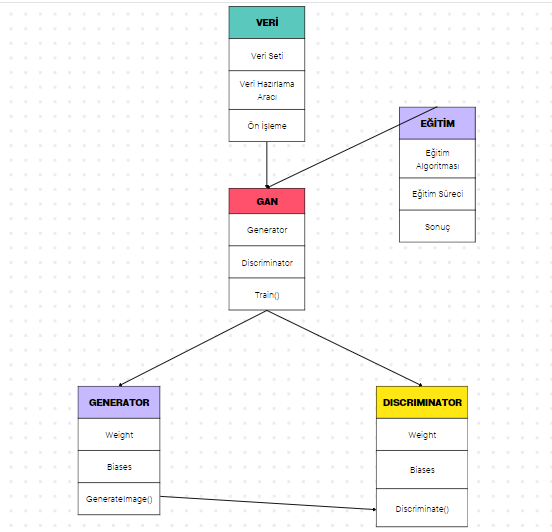
\includegraphics[width=1\textwidth]{uml}
		\label{uml}
		Şekil \ref{uml}: UML Şeması
		
		\item \textbf{Tartışma Planı}
		\\Projede elde edilen sonuçlar, yapay zeka destekli yüz oluşturma tekniklerinin potansiyelini ve sınırlamalarını vurgulamak için analiz edilecektir. Modelin başarıları ve zorlukları belirlenecek ve özellikle modelin belirli demografik gruplara karşı önyargılı olma sorunu tartışılacaktır. Ayrıca, etik ve mahremiyet konuları da tartışma kapsamında ele alınacaktır, çünkü bu teknoloji kötü niyetli amaçlar için de kullanılabilir. Gelecekteki çalışmalar, bu tür sorunları ele alarak yapay zeka destekli yüz oluşturma tekniklerinin daha güvenli ve etik bir şekilde kullanılmasını sağlamayı amaçlayacaktır.
		\item \textbf{Veri Toplama}
		\\Yüz oluşturma projesi için gerekli veri setlerini toplamak için çeşitli kaynaklar araştırılacak ve uygun veri setleri seçilecektir. Bu veri setleri, farklı ırklardan, yaş gruplarından ve cinsiyetlerden insan yüzlerini içermektedir. Amacım, projemin geniş bir yelpazede kullanılabilir ve temsil edici olmasını sağlamaktır. Toplanan veri setleri, toplamda 100.000'den fazla yüz görüntüsünü kapsaması hedeflenmektedir. Bu çeşitlilik, modelin etkinliğini artırarak daha geniş bir kullanıcı kitlesine hitap etmesine olanak tanıyacaktır. Yüzlerin çeşitli özelliklerini içeren bu geniş veri setleri, modelin eğitimini ve sonuçlarının doğruluğunu artırarak, gerçek dünya koşullarında daha başarılı sonuçlar elde etmemizi sağlayacaktır.
		
		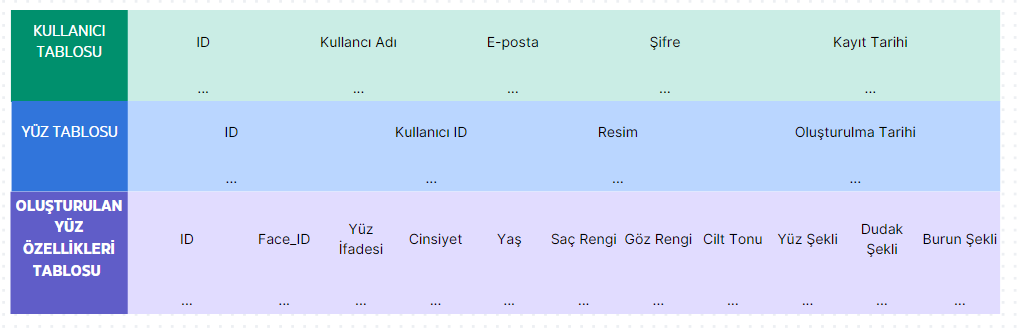
\includegraphics[width=1\textwidth]{veritabanıtasarımı}
		\label{veritabanıtasarımı}
		Şekil \ref{veritabanıtasarımı}:Veri Tabanı Tasarımı
		\item \textbf{Veri Ön İşleme}
		\\ Toplanan veri setleri, öncelikle boyutlandırılacak, normalize edilecek ve gereksiz gürültülerden arındırılacaktır. Ardından, yüzlerin manuel olarak hizalanması ve etiketlenmesi yapılacaktır. Veri seti, eğitim, doğrulama ve test setleri olarak bölünecek, böylece modelin performansı objektif bir şekilde değerlendirilebilecektir.
		\item \textbf{Model}
		\\Proje kapsamında kullanılacak model, StyleGAN3 veya benzeri bir GAN modelleri ile örnek uygulamalar yapılacak. Bu model, yüksek çözünürlüklü ve gerçekçi görüntüler üretme yeteneği ile öne çıkan bir modeldir. Modeller, proje ilerledikçe daha kapsamlı bir literatür incelemesi ve karşılaştırmalı analiz yapılarak incelenecektir. Aynı zamanda kendim modelin eğitimine başlamış olacağım. Bir yandan yapılmış farklı yöntemlerle modellerin sonuçlarını incelerken bir yandan da farklı bir yolla kendim eğitecek ve onu deneyeceğim.
		\item \textbf{Model Eğitimi}
		\\Model, toplanan veri setleri üzerinde eğitilecektir. Eğitim sürecinde, modelin generative ve discriminative ağları arasındaki rekabetçi dinamiklerin optimize edilmesi için uygun kayıp fonksiyonları ve optimizasyon algoritmaları kullanılacaktır. Modelin eğitimi, belirlenen epoch sayısı veya başka bir performans ölçütüne ulaşıncaya kadar devam edecektir.
		\item \textbf{Model Değerlendirmesi}
		\\Eğitilen model, gerçekçi ve inandırıcı yüzler üretebilmeli ve veri seti üzerinde iyi performans göstermelidir. Modelin doğruluğu, çeşitli ölçütler ve metrikler kullanılarak değerlendirilecek ve gerektiğinde ayarlamalar yapılacaktır.
		
		\includegraphics[width=1\textwidth]{BLOKDİYAGRAMI}
		\label{BLOKDİYAGRAMI}
		Şekil \ref{BLOKDİYAGRAMI}: Blok Diyagramı
		\item\textbf{ Sonuçların Analizi}
		\\Eğitilen modelin performansı analiz edilecek ve elde edilen sonuçlar raporlanacaktır. Sonuçlar, üretilen yüzlerin kalitesi, doğruluğu ve çeşitliliği gibi faktörlere göre değerlendirilecek ve mevcut literatürle karşılaştırılacaktır.
		
		
		
		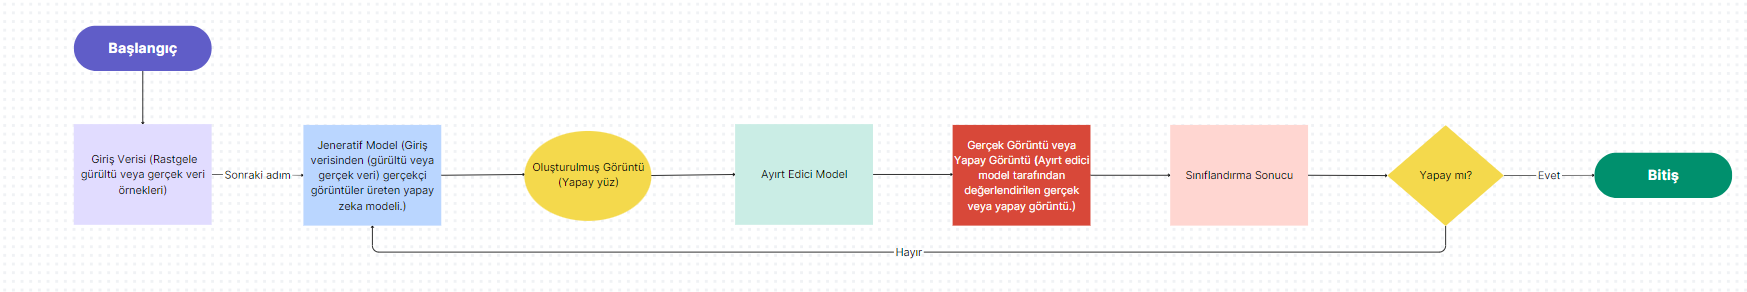
\includegraphics[width=1\textwidth]{işakışşeması}
		\label{işakışşeması}
		Şekil \ref{işakışşeması}: İş Akış Şeması
	\end{enumerate}
\begin{center}
		\section{Veriler}
\end{center}
	\begin{flushleft}
		Bu çalışma GAN yöntemi kullanılarak gerçekleştirilecek olan yüz oluşturma işleminin yapılması üzerinedir. Bu çalışma için CelebA\cite{CelebAMask-HQ} veri setinden rastgele seçilecek eşit sayıda kadın ve erkek verileri ile eğitimin gerçekleşmesi planlanmaktadır. Veri seçimi kısmı metodolojide detaylıca anlatılmıştı.
		Kod için örnek çalışmalarda Google Colab kullanılırken yazılacak kodun Anaconda Jupiter Notebook'ta yazılması planlanmaktadır. 
		
		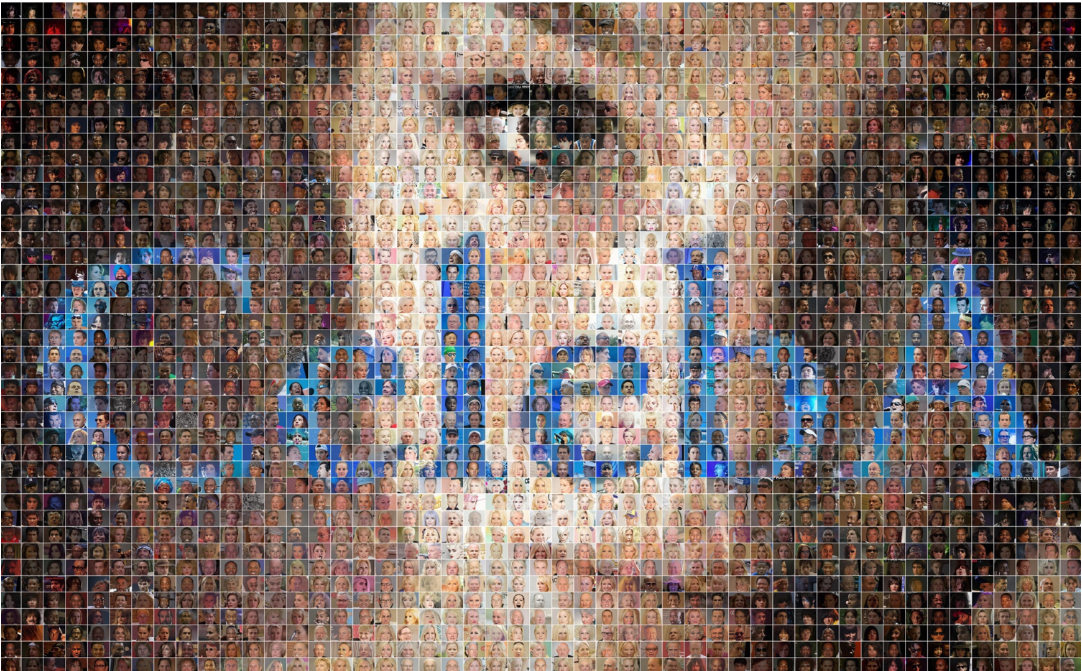
\includegraphics[width=1\textwidth]{abc}
	\end{flushleft}
\begin{center}
		\section{Sonuç}
\end{center}
	\begin{flushleft}
		Projenin başlıca hedefleri yüksek çözünürlüklü ve gerçekçi insan yüzlerinin üretimi için yapay zeka destekli bir model geliştirmek, modelin çeşitli demografik gruplara karşı önyargısız ve genelleyici olmasını sağlamak, modelin etik ve mahremiyet standartlarına uygun bir şekilde çalışmasını sağlamak olarak belirledim.
	Projenin başarıyla tamamlanması durumunda beklenen sonuç ve planlanan çıktı olarak yüksek kaliteli ve gerçekçi insan yüzleri üreten bir yapay zeka modeli geliştirmiş olmak, modelin çeşitli demografik gruplara karşı önyargısız olduğu ve genel geçerli olduğunu göstermek, mahremiyet standartlarına uygun bir şekilde çalışan bir model oluşturabilmek olarak belirledim.
	
	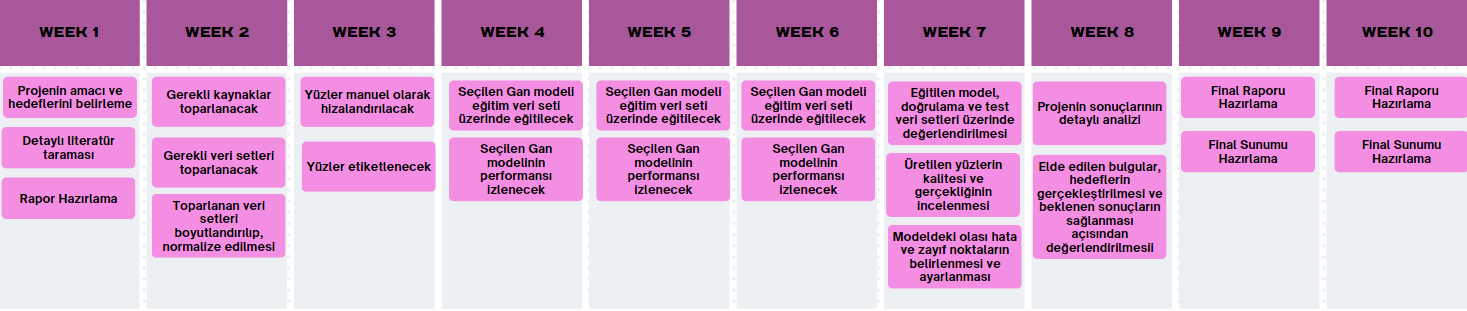
\includegraphics[width=1\textwidth]{ganntchart}
	\label{ganntchart}
	Şekil \ref{ganntchart}: Gannt Şeması
	\newpage
	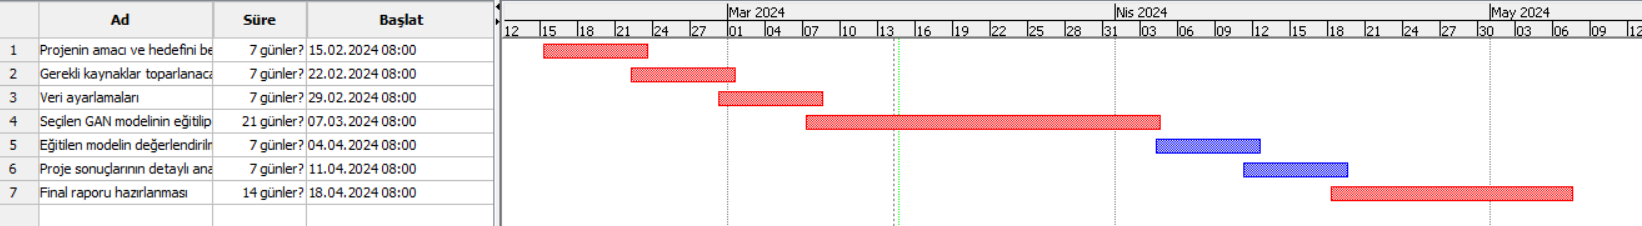
\includegraphics[width=1\textwidth]{2ganttchart}
	\label{2ganttchart}
	Şekil \ref{2ganttchart}: Gannt Şeması
	
	
	\textbf{İş Paketleri Tanımı}
	
	\textit{Projenin amacı ve hedefini belirleme:} Detaylı literatür taraması, rapor hazırlama.
	
    \textit{Gerekli kaynaklar toparlanacak:} Gerekli veri setleri toparlanacak, toparlanan veri setlerinin boyutlandırılıp, normalize edilmesi.
	
	\textit{Veri ayarlamaları:} Yüzler manuel olarak hizalandırılacak ve yüzler etiketlenecek.
	
	\textit{Seçilen GAN modelinin eğitilip izlenmesi:} Seçilen GAN modeli eğitim veri seti üzerinde eğitilecek, seçilen GAN modelinin performansının izlenmesi.
    
    \textit{Eğitilen modelin değerlendirilmesi:} Eğitilen model, doğrulama ve test veri setleri üzerinde değerlendirilmesi, üretilen yüzlerin kalitesinin ve gerçekliğinin incelenmesi, modeldeki olası hata ve zayıf noktaların belirlenmesi ve ayarlanması.
	
	\textit{Proje sonuçlarının detaylı analizi:} Proje sonuçlarının detaylı analizi, elde edilen bulgular ve hedeflerin gerçekleştirilmesi ve beklenen sonuçların sağlanması açısından değerlendirilmesi.
	
	\textit{Final raporu hazırlanması:} Final rapor ve sunumunun hazırlanması.
	\newpage
	\end{flushleft}
	\begin{center}
		\bibliographystyle{ieeetr}
	\bibliography{IEEEreferences.bib}
	\end{center}
\end{document}